\documentclass[../main]{subfiles}
\begin{document}
\chapter{Expectation--Maximization and Mixture of Gaussians}
\begin{introduction}
    \item Mixture of Gaussians (MoG) as a generative clustering model
    \item Maximum likelihood with latent variables: why it is hard
    \item KL divergence and the evidence lower bound (ELBO)
    \item EM algorithm: E-step and M-step, monotonic improvement and local optima
    \item Closed-form EM updates for MoG and the connection to K-means
\end{introduction}

\section{Mixture of Gaussians (MoG): a generative view of clustering}
We revisit clustering from a probabilistic and generative perspective.
Instead of assigning each datapoint to a cluster deterministically, we assume
each datapoint is generated by \emph{first} choosing a latent cluster index and
\emph{then} sampling from a Gaussian distribution attached to that cluster.

\subsection{Latent variable and generative process}
Let $K\in\mathbb N$ be the number of clusters (components). For each datapoint
$x\in\mathbb R^d$, introduce a latent discrete variable
\begin{equation}
    G \in \{1,2,\dots,K\},
\end{equation}
where $G=k$ indicates that $x$ is generated from the $k$-th Gaussian component.
We model
\begin{equation}
    p(G=k)=\pi_k,\qquad \pi_k\ge 0,\qquad \sum_{k=1}^K \pi_k = 1,
\end{equation}
and the conditional likelihood
\begin{equation}
    p(x\mid G=k)=\mathcal N(x\mid \mu_k,\Sigma_k),
\end{equation}
where $\mu_k\in\mathbb R^d$ and $\Sigma_k\in\mathbb R^{d\times d}$ is symmetric
positive definite.

\begin{note}
    Earlier chapters may encode the latent cluster by a one-hot vector
    $z\in\{0,1\}^K$ with $\sum_k z_k=1$.  The integer notation here is
    equivalent but notationally lighter:
    $G=k \Longleftrightarrow z_k=1$.
\end{note}

\subsection{Marginal likelihood and the MLE objective}
By marginalizing $G$, the density of $x$ becomes a mixture:
\begin{equation}\label{eq:mog-marginal}
    p(x;\theta)
    =
    \sum_{k=1}^K p(G=k)\,p(x\mid G=k)
    =
    \sum_{k=1}^K \pi_k\,\mathcal N(x\mid \mu_k,\Sigma_k),
\end{equation}
where we collect all parameters as
\begin{equation}
    \theta := \Bigl\{\pi_k,\mu_k,\Sigma_k\Bigr\}_{k=1}^K.
\end{equation}

Given i.i.d.\ data $\{x_i\}_{i=1}^n$, maximum likelihood estimation solves
\begin{equation}\label{eq:mog-mle}
    \argmax_{\theta}\;
    \sum_{i=1}^n \log p(x_i;\theta)
    =
    \argmax_{\theta}\;
    \sum_{i=1}^n
    \log\!\left(
        \sum_{k=1}^K \pi_k\,\mathcal N(x_i\mid \mu_k,\Sigma_k)
    \right).
\end{equation}

\begin{remark}
    Unlike supervised learning objectives of the form $\sum_i \log p(y_i\mid
    x_i;\theta)$, unsupervised density estimation maximizes $\sum_i \log
    p(x_i;\theta)$ directly because no labels are observed.
\end{remark}

\subsection{Why direct optimization is non-trivial}
The objective \eqref{eq:mog-mle} is difficult for at least two reasons.
\begin{itemize}
    \item \textbf{Log-sum structure:} $\log\big(\sum_k \pi_k \mathcal N(\cdot)\big)$
    couples all components inside a logarithm, preventing simple closed-form
    derivatives from decoupling.
    \item \textbf{Constraints:} $\{\pi_k\}$ must lie on the simplex and each
    $\Sigma_k$ must be positive definite. One can use constrained optimization,
    penalty methods, or reparameterization, but a naive unconstrained gradient
    method is not directly applicable.
\end{itemize}
\begin{remark}
    Gradient descent can be made to work with non-trivial adaptations (e.g.,
    softmax parameters for $\pi$, Cholesky factors for $\Sigma$), but EM
    typically provides a faster and more elegant framework for this class of
    latent-variable MLE problems.
\end{remark}

\section{From latent-variable MLE to ELBO}
We now derive the Expectation--Maximization (EM) algorithm in a general setting.

\subsection{General latent-variable likelihood}
Let $x$ be observed and $z$ be a latent variable (discrete or continuous).
Assume a joint model $p(x,z;\theta)$. The marginal likelihood is
\begin{equation}
    p(x;\theta) = \sum_z p(x,z;\theta)\qquad
    (\text{or } \int p(x,z;\theta)\,\mathrm dz).
\end{equation}
In MLE, the objective is
\begin{equation}
    \argmax_{\theta}\; \sum_{i=1}^n \log p(x_i;\theta).
\end{equation}
The marginalization over $z$ often makes $\log p(x;\theta)$ hard to optimize.

\subsection{KL divergence: definition and key properties}
\begin{definition}[Kullback--Leibler divergence]
    For distributions $Q$ and $P$ on the same variable $Z$, the KL divergence
    is
    \begin{equation}
        \mathrm{KL}(Q\|P)
        := \mathbb E_{Z\sim Q}\!\left[\log\frac{Q(Z)}{P(Z)}\right].
    \end{equation}
\end{definition}

\begin{proposition}[Basic properties of KL]\label{prop:kl-basic}
    For any $Q,P$,
    \begin{enumerate}
        \item $\mathrm{KL}(Q\|P)\ge 0$.
        \item $\mathrm{KL}(Q\|P)=0$ if and only if $Q=P$ almost surely.
        \item In general, $\mathrm{KL}(Q\|P)\neq \mathrm{KL}(P\|Q)$ (not symmetric).
    \end{enumerate}
\end{proposition}
\begin{proof}
    By Jensen's inequality applied to the convex function $-\log(\cdot)$,
    \begin{align*}
        \mathrm{KL}(Q\|P)
        &= -\mathbb E_{Q}\!\left[\log \frac{P(Z)}{Q(Z)}\right]
        \ge -\log \mathbb E_{Q}\!\left[\frac{P(Z)}{Q(Z)}\right]
        = -\log\!\left(\sum_z P(z)\right)
        = 0,
    \end{align*}
    and equality holds iff $\frac{P(Z)}{Q(Z)}$ is constant $Q$-a.s., which gives
    $Q=P$ a.s.  Non-symmetry follows from counterexamples.
\end{proof}

\begin{remark}
    KL can be written as \textbf{cross-entropy minus entropy}:
    \begin{equation}
        \mathrm{KL}(Q\|P)
        =
        \underbrace{\mathbb E_Q[-\log P(Z)]}_{\text{cross-entropy}}
        -
        \underbrace{\mathbb E_Q[-\log Q(Z)]}_{\text{entropy}}.
    \end{equation}
    This explains why using the ``wrong code'' $P$ to encode samples from $Q$
    necessarily incurs extra expected description length.
\end{remark}

\subsection{ELBO decomposition}
Introduce an arbitrary distribution $q(z)$ (a ``variational distribution'').
Then the following identity holds:
\begin{theorem}[ELBO decomposition]\label{thm:elbo}
    For any $q(z)$ and any $\theta$,
    \begin{equation}\label{eq:elbo-decomp}
        \log p(x;\theta)
        =
        \underbrace{
        \mathbb E_{z\sim q}\!\left[\log \frac{p(x,z;\theta)}{q(z)}\right]
        }_{\mathcal L(q,\theta)\;\;(\text{ELBO})}
        +
        \underbrace{
        \mathrm{KL}\!\left(q(z)\,\middle\|\,p(z\mid x;\theta)\right)
        }_{\ge 0}.
    \end{equation}
    Consequently, $\mathcal L(q,\theta)\le \log p(x;\theta)$ for all $q$.
\end{theorem}
\begin{proof}
    Starting from $\log p(x;\theta)$ and taking expectation over $q$,
    \begin{align*}
        \log p(x;\theta)
        &= \sum_z q(z)\,\log p(x;\theta) \\
        &= \sum_z q(z)\,\log \frac{p(x,z;\theta)}{p(z\mid x;\theta)} \\
        &= \sum_z q(z)\,\log \frac{p(x,z;\theta)}{q(z)}
        + \sum_z q(z)\,\log \frac{q(z)}{p(z\mid x;\theta)},
    \end{align*}
    where the last term is exactly the KL divergence.
\end{proof}

\begin{definition}[Evidence lower bound (ELBO)]
    The functional
    \begin{equation}
        \mathcal L(q,\theta)
        :=
        \mathbb E_{z\sim q}\!\left[\log p(x,z;\theta)\right]
        -
        \mathbb E_{z\sim q}\!\left[\log q(z)\right]
        =
        \mathbb E_{z\sim q}\!\left[\log \frac{p(x,z;\theta)}{q(z)}\right]
    \end{equation}
    is called the \emph{evidence lower bound}.
\end{definition}

\begin{remark}
    The abbreviation \textbf{ELBO} is commonly read as ``elbow'' in talks.
    The bound gap is precisely
    $\mathrm{KL}\big(q(z)\|p(z\mid x;\theta)\big)$.
    When $q(z)=p(z\mid x;\theta)$, the bound is tight.
\end{remark}

\begin{note}
    When the posterior $p(z\mid x;\theta)$ is intractable, one typically
    restricts $q$ to a tractable family and maximizes ELBO approximately (this
    is the core idea of variational inference). EM can be viewed as the special
    case where the E-step posterior is tractable and makes the bound tight at
    the current iterate.
\end{note}

\section{The EM algorithm}
EM is an iterative algorithm that alternates between optimizing $q$ (E-step)
and optimizing $\theta$ (M-step), using ELBO as a surrogate objective.

\subsection{E-step and M-step from ELBO}
Suppose we are at $\theta^{(t)}$.
\begin{itemize}
    \item \textbf{E-step (fix $\theta$):}
    choose $q^{(t+1)}$ to maximize $\mathcal L(q,\theta^{(t)})$.
    Since $\log p(x;\theta^{(t)})$ is a constant w.r.t.\ $q$,
    Theorem~\ref{thm:elbo} implies
    \begin{equation}\label{eq:e-step}
        q^{(t+1)}(z)
        =
        p\bigl(z\mid x;\theta^{(t)}\bigr),
    \end{equation}
    which minimizes the KL gap to $0$.

    \item \textbf{M-step (fix $q$):}
    update $\theta$ by maximizing the ELBO
    \begin{equation}\label{eq:m-step}
        \theta^{(t+1)}
        \in
        \argmax_{\theta}\; \mathcal L\!\left(q^{(t+1)},\theta\right).
    \end{equation}
    Because the term $-\mathbb E_{q^{(t+1)}}[\log q^{(t+1)}(z)]$ does not depend
    on $\theta$, the M-step equivalently maximizes
    \begin{equation}\label{eq:q-function}
        Q(\theta\mid \theta^{(t)})
        :=
        \mathbb E_{z\sim p(z\mid x;\theta^{(t)})}\!\left[\log p(x,z;\theta)\right],
    \end{equation}
    the expected complete-data log-likelihood.
\end{itemize}

\begin{remark}
    The ``expectation'' in \textbf{E-step} refers to taking expectation with
    respect to the posterior $p(z\mid x;\theta^{(t)})$, which is computed in the
    E-step and then used to form the expected complete log-likelihood in the
    M-step.
\end{remark}

\begin{note}
    The overall algorithm repeats \textbf{E-step $\rightarrow$ M-step} until
    convergence, e.g.\ until $\theta^{(t+1)}$ is sufficiently close to
    $\theta^{(t)}$ or the log-likelihood improvement becomes negligible.
\end{note}

\subsection{Monotonicity and local optima}
\begin{proposition}[Monotonic improvement]
    Each EM iteration does not decrease the data log-likelihood:
    \[
        \log p(x;\theta^{(t+1)}) \ge \log p(x;\theta^{(t)}).
    \]
\end{proposition}
\begin{proof}
    In the E-step, the ELBO is made tight at $\theta^{(t)}$ by choosing
    $q^{(t+1)}(z)=p(z\mid x;\theta^{(t)})$, hence
    $\mathcal L(q^{(t+1)},\theta^{(t)})=\log p(x;\theta^{(t)})$.
    In the M-step, we maximize the ELBO in $\theta$, so
    \[
        \mathcal L(q^{(t+1)},\theta^{(t+1)})
        \ge
        \mathcal L(q^{(t+1)},\theta^{(t)})
        =
        \log p(x;\theta^{(t)}).
    \]
    Since ELBO is always a lower bound, $\log p(x;\theta^{(t+1)})\ge
    \mathcal L(q^{(t+1)},\theta^{(t+1)})$, proving the claim.
\end{proof}

\begin{remark}
    EM typically converges to a \emph{stationary point}, which may be a local
    optimum. Different initializations can lead to different solutions.
\end{remark}

% \begin{figure}[h]
%     \centering
%     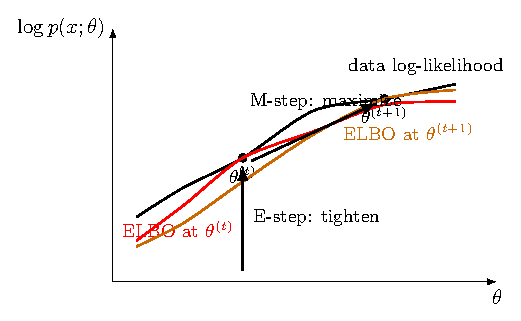
\includegraphics[width=0.9\textwidth]{../../mvp/tikz/9/5.pdf}
%     \caption{Geometric intuition: each E-step picks an ELBO that ``touches'' the log-likelihood at the current $\theta^{(t)}$, and the M-step maximizes that ELBO to obtain a new parameter $\theta^{(t+1)}$ with increased likelihood.}
%     \label{fig:em-elbo-geometry}
% \end{figure}

\section{EM for Mixture of Gaussians}
We now apply the general EM framework to MoG.

\subsection{Complete-data likelihood}
For a single datapoint $(x_i,G_i)$,
\begin{equation}
    p(x_i,G_i=k;\theta)
    =
    p(G_i=k)\,p(x_i\mid G_i=k)
    =
    \pi_k\,\mathcal N(x_i\mid \mu_k,\Sigma_k).
\end{equation}
For the dataset, the complete-data log-likelihood is
\begin{equation}
    \log p(\{x_i\},\{G_i\};\theta)
    =
    \sum_{i=1}^n \sum_{k=1}^K \mathbb I\{G_i=k\}
    \Bigl(
        \log \pi_k + \log \mathcal N(x_i\mid \mu_k,\Sigma_k)
    \Bigr).
\end{equation}

\subsection{E-step: responsibilities}
Define the \emph{responsibility} (posterior assignment probability)
\begin{equation}\label{eq:responsibility}
    \gamma_{ik}
    :=
    p(G_i=k \mid x_i;\theta^{(t)}).
\end{equation}
By Bayes' rule,
\begin{equation}\label{eq:mog-e-step}
    \gamma_{ik}
    =
    \frac{
        \pi_k^{(t)}\,\mathcal N(x_i\mid \mu_k^{(t)},\Sigma_k^{(t)})
    }{
        \sum_{j=1}^K \pi_j^{(t)}\,\mathcal N(x_i\mid \mu_j^{(t)},\Sigma_j^{(t)})
    }.
\end{equation}
Intuitively, $\gamma_{ik}$ measures the fraction of ``credit'' component $k$
takes for explaining datapoint $x_i$.

\subsection{M-step: closed-form updates}
Given $\{\gamma_{ik}\}$, the EM objective for MoG becomes
\begin{equation}\label{eq:mog-Q}
    Q(\theta\mid \theta^{(t)})
    =
    \sum_{i=1}^n \sum_{k=1}^K \gamma_{ik}
    \Bigl(
        \log \pi_k + \log \mathcal N(x_i\mid \mu_k,\Sigma_k)
    \Bigr).
\end{equation}
Let
\begin{equation}
    N_k := \sum_{i=1}^n \gamma_{ik}.
\end{equation}

\subsubsection{Update of $\pi_k$ (simplex constraint)}
We maximize \eqref{eq:mog-Q} w.r.t.\ $\pi$ subject to $\sum_k \pi_k=1$.
Introduce a Lagrange multiplier $\lambda$:
\begin{equation}
    \mathcal J(\pi,\lambda)
    =
    \sum_{i=1}^n \sum_{k=1}^K \gamma_{ik}\log \pi_k
    + \lambda\left(1-\sum_{k=1}^K \pi_k\right).
\end{equation}
Setting $\partial \mathcal J/\partial \pi_k=0$ gives
\begin{equation}
    \pi_k
    =
    \frac{1}{n}\sum_{i=1}^n \gamma_{ik}
    =
    \frac{N_k}{n}.
\end{equation}

\subsubsection{Update of $\mu_k$}
Using the Gaussian log-density, the terms depending on $\mu_k$ yield the
weighted least-squares problem whose solution is
\begin{equation}\label{eq:mog-mu-update}
    \mu_k
    =
    \frac{\sum_{i=1}^n \gamma_{ik} x_i}{\sum_{i=1}^n \gamma_{ik}}
    =
    \frac{1}{N_k}\sum_{i=1}^n \gamma_{ik} x_i.
\end{equation}

\subsubsection{Update of $\Sigma_k$}
Similarly, maximizing w.r.t.\ $\Sigma_k$ gives
\begin{equation}\label{eq:mog-sigma-update}
    \Sigma_k
    =
    \frac{\sum_{i=1}^n \gamma_{ik} (x_i-\mu_k)(x_i-\mu_k)^\top}{\sum_{i=1}^n \gamma_{ik}}
    =
    \frac{1}{N_k}\sum_{i=1}^n \gamma_{ik} (x_i-\mu_k)(x_i-\mu_k)^\top.
\end{equation}

\begin{remark}
    The updates \eqref{eq:mog-mu-update}--\eqref{eq:mog-sigma-update} are
    \textbf{soft-assignment weighted} empirical mean and covariance.  If
    $\gamma_{ik}\in\{0,1\}$ becomes hard assignment, they reduce to the usual
    sample mean/covariance of points in cluster $k$.
\end{remark}

\subsection{Relationship to K-means as a limiting case}
Assume an isotropic shared covariance $\Sigma_k=\sigma^2 I$ for all $k$.
Then
\begin{equation}
    \gamma_{ik}
    \propto
    \pi_k \exp\left(-\frac{\|x_i-\mu_k\|^2}{2\sigma^2}\right).
\end{equation}
As $\sigma\to 0$, the softmax distribution concentrates on the closest mean:
\begin{equation}
    \gamma_{ik}
    \to
    \begin{cases}
        1, & k=\argmin_j \|x_i-\mu_j\|^2,\\
        0, & \text{otherwise},
    \end{cases}
\end{equation}
which recovers the hard assignment step of K-means. With these hard assignments,
the M-step mean update reduces to the K-means centroid update.

\begin{remark}
    This connection explains a common interpretation: \textbf{K-means is a
    special/limiting case of MoG} (and can be seen as a degenerate EM).
\end{remark}

\section{A clarification: PCA vs regression (from Q\&A)}
\begin{note}
    PCA is an \emph{unsupervised} problem: all coordinates are treated
    symmetrically and the objective is to find a low-dimensional subspace that
    best explains the variance/geometry of $x$.
    In contrast, regression is \emph{supervised}: $y$ plays a special role and
    the objective is to minimize prediction error of $y$ given $x$.
    Therefore, even if one augments $x$ with $y$, the resulting optimization is
    not equivalent to PCA because the symmetry between coordinates is broken by
    the learning objective.
\end{note}

\end{document}


